% !TEX TS-program = xelatex
% !TEX encoding = UTF-8 Unicode
% !Mode:: "TeX:UTF-8"

%This file contains the LaTeX code of my laboratory report for my ICS II course.
%Author: 张作柏/Zuobai Zhang <17300240035@fudan.edu.cn>

% This is a simple template for a LaTeX document using the "article" class.
% See "book", "report", "letter" for other types of document.

\documentclass[12pt]{article} % use larger type; default would be 10pt

\usepackage[utf8]{inputenc} % set input encoding (not needed with XeLaTeX)

%%% Examples of Article customizations
% These packages are optional, depending whether you want the features they provide.
% See the LaTeX Companion or other references for full information.

%%% PAGE DIMENSIONS
\usepackage[top=1.05in, bottom=0.95in, left=0.90in, right=1.10in]{geometry}
%\usepackage{geometry} % to change the page dimensions
\geometry{a4paper} % or letterpaper (US) or a5paper or....
% \geometry{margin=2in} % for example, change the margins to 2 inches all round
% \geometry{landscape} % set up the page for landscape
%   read geometry.pdf for detailed page layout information

\usepackage{graphicx} % support the \includegraphics command and options

% \usepackage[parfill]{parskip} % Activate to begin paragraphs with an empty line rather than an indent

%%% PACKAGES
\usepackage{booktabs} % for much better looking tables
\usepackage{array} % for better arrays (eg matrices) in maths
\usepackage{paralist} % very flexible & customisable lists (eg. enumerate/itemize, etc.)
\usepackage{verbatim} % adds environment for commenting out blocks of text & for better verbatim
\usepackage{subfig} % make it possible to include more than one captioned figure/table in a single float
% These packages are all incorporated in the memoir class to one degree or another...

%%% HEADERS & FOOTERS
\usepackage{fancyhdr} % This should be set AFTER setting up the page geometry
\pagestyle{fancy} % options: empty , plain , fancy
%\renewcommand{\headrulewidth}{0pt} % customise the layout...
\lhead{}\chead{}\rhead{}
\lfoot{}\cfoot{\thepage}\rfoot{}

%%% SECTION TITLE APPEARANCE
\usepackage{sectsty}
\allsectionsfont{\sffamily\mdseries\upshape} % (See the fntguide.pdf for font help)
% (This matches ConTeXt defaults)

%%% ToC (table of contents) APPEARANCE
\usepackage[nottoc,notlof,notlot]{tocbibind} % Put the bibliography in the ToC
\usepackage[titles,subfigure]{tocloft} % Alter the style of the Table of Contents
\renewcommand{\cftsecfont}{\rmfamily\mdseries\upshape}
\renewcommand{\cftsecpagefont}{\rmfamily\mdseries\upshape} % No bold!
\usepackage{titletoc}
\titlecontents{section}
              [1.5cm]
              {\bf \large}%
              {\contentslabel{1.8em}}%
              {}%
              {\titlerule*[0.5pc]{$\cdot$}\contentspage\hspace*{0.6cm}}%
		   [\vspace{0.5em}]
\titlecontents{subsection}
              [1.8cm]
              {\normalsize}%
              {\contentslabel{2.0em}}%
              {}%
              {\titlerule*[0.5pc]{$\cdot$}\contentspage\hspace*{0.6cm}}%
		   [\vspace{0.4em}]
\titlecontents{subsubsection}
              [2.1cm]
              {\small}%
              {\contentslabel{2.5em}}%
              {}%
              {\titlerule*[0.5pc]{$\cdot$}\contentspage\hspace*{0.6cm}}%
		   [\vspace{0.4em}]


\usepackage[UTF8]{ctex}
\usepackage{fancyhdr}
\usepackage{enumerate}
\usepackage{indentfirst}
\usepackage{extramarks}
\usepackage{titling}
\usepackage{listings}
\usepackage{xcolor}
\usepackage{fontspec}
\usepackage[CJKbookmarks=true,colorlinks,linkcolor=black]{hyperref}
\setmainfont{Times New Roman}



\definecolor{mygreen}{rgb}{0,0.6,0}  
\definecolor{mygray}{rgb}{0.9,0.9,0.9}  
\definecolor{mymauve}{rgb}{0.58,0,0.82}  
  
\lstset{ %  
  backgroundcolor=\color{mygray},   % choose the background color; you must add \usepackage{color} or \usepackage{xcolor}  
  basicstyle=
	{
		\footnotesize
		\fontspec{Consolas}
	},        % the size of the fonts that are used for the code  
  breakatwhitespace=false,         % sets if automatic breaks should only happen at whitespace  
  breaklines=true,                 % sets automatic line breaking  
  captionpos=bl,                    % sets the caption-position to bottom  
  commentstyle=
	{
		\color{mygray}
		\fontspec{Consolas Italic}
	},    % comment style  
  deletekeywords={...},            % if you want to delete keywords from the given language  
  escapeinside={\%*}{*)},          % if you want to add LaTeX within your code  
  extendedchars=true,              % lets you use non-ASCII characters; for 8-bits encodings only, does not work with UTF-8  
  %frame=shadow,                    % adds a frame around the code  
  keepspaces=true,                 % keeps spaces in text, useful for keeping indentation of code (possibly needs columns=flexible)  
  keywordstyle=
	{
		\color{blue}
		\fontspec{Consolas Bold}
	},       % keyword style  
  %language=Python,                 % the language of the code  
  morekeywords={*,...},            % if you want to add more keywords to the set  
  numbers=none,                    % where to put the line-numbers; possible values are (none, left, right)  
  numbersep=5pt,                   % how far the line-numbers are from the code  
  numberstyle=\tiny\color{mygray}, % the style that is used for the line-numbers  
  rulecolor=\color{black},         % if not set, the frame-color may be changed on line-breaks within not-black text (e.g. comments (green here))  
  showspaces=false,                % show spaces everywhere adding particular underscores; it overrides 'showstringspaces'  
  showstringspaces=false,          % underline spaces within strings only  
  showtabs=false,                  % show tabs within strings adding particular underscores  
  stepnumber=1,                    % the step between two line-numbers. If it's 1, each line will be numbered  
  stringstyle=\color{blue},     % string literal style  
  tabsize=4,                       % sets default tabsize to 2 spaces  
  %title=myPython.py                   % show the filename of files included with \lstinputlisting; also try caption instead of title  
}  


%%% END Article customizations

%%% The "real" document content comes below...

%\title{\textbf{Digital Logic and Computer Design Report}}
\title{\textbf{Cache设计实验报告}}
\author{张作柏\\17300240035}
%\date{} % Activate to display a given date or no date (if empty),
         % otherwise the current date is printed 

\begin{document}
\begin{sloppypar}
\maketitle

\pagestyle{fancy}
\lhead{\textbf{{\thetitle}}}
\rhead{\textbf{\nouppercase{\firstleftmark}}}
\cfoot{\thepage}

\thispagestyle{empty}
\tableofcontents
\clearpage

\setcounter{page}{1}

\section{缓存机制简介}

计算机的主存一般由DRAM芯片构成。在过去的30年中,DRAM的速度仅以每年7\%增长,而处理器的性能则以每年25\%\~{} 50\%增长。在1980年前后,处理器和存储器的速度是一样的,但是性能从那时开始有了差别,存储器速度开始严重落后。DRAM访问时间比处理器周期长一到两个数量级。

为了抵消这种趋势,计算机将最常用的指令和数据存储在更快但更小的存储器中,这种存储器称为{\em 高速缓存}(cache),其速度与处理器相近,但是容量较小。如果处理器需要的数据在高速缓存中可用,那么它可以快速返回,这成为缓存命中(hit),否则,处理器就需要从主存(DRAM)中获得数据,这称为缓存缺失(miss)。如果在大部分情况下缓存命中,那么处理器就基本上不需要等待低速的主存。


\subsection{高速缓存原理}

高速缓存主要应用了{\em 时间局部性}和{\em 空间局部性}的原理。时间局部性意味着最近使用过的数据可能很快就会被再次使用。而空间局部性意味着当使用一个数据时,很可能会在之后使用与其相邻的数据。

高速缓存可以一次从主存中取许多相邻的数据,以此利用空间局部性。同时,还可以根据之前的数据使用情况,选择合适的预取策略。而cache对时间局部性的利用主要体现在保存之前使用的数据和数据替换策略的设计。我们将在接下来的两小节分别进行讨论。

\subsection{高速缓存结构}

高速缓存通常保存存储器数据,其存放数据字的数量称为{\em 容量}($C$)。

为了利用空间局部性,当处理器访问一块数据时,我们可以从内存中提取多个相邻的字。这样的一组字称为{\em 高速缓存块}(cache block),一个高速缓存块中的字数称为{\em 块大小}($b$),容量为C的高速缓存包含了$B=C/b$个块。

一个高速缓存可以组织成$S$组,其中每一组有一个或多个数据块。主存中数据的地址和高速缓存中数据的位置之间的关系称为{\em 映射}(mapping)。高速缓存按照组中块的数量进行分类:
\begin{itemize}
\item {\bf 直接映射}: 每组内只有一块,所以组数$S=B$。在这种情况下,数据替换策略是无意义的。
\item {\bf 多路组相联}: 每组提供$N$块,此时需满足$S\times N=B$。每个内存地址可以映射到唯一的组中,但是它可以映射到一组中$N$块的任意一块。
\item {\bf 全相联}: 只包含一组,即$S=1$。这一组中包含了$B$路,存储器地址可以映射到这些路中的任何一块。
\end{itemize}

\begin{figure}[h]
\centering
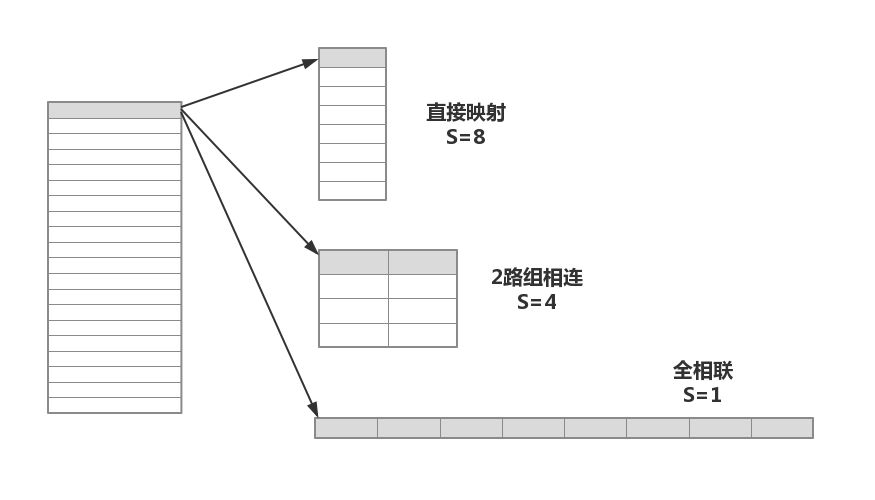
\includegraphics[width =\linewidth]{figure/Cachearch.jpg}
\caption{Cache组织形式:直接映射、多路组相连和全相联}
\label{fig:arch}
\end{figure}

图~\ref{fig:arch}简单地展示了三种组织形式,其中灰色的部分对应该内存地址可能映射到的块。注意到,以上三种组织形式是本质相同的,只是参数的设置不同而已,所以在书写代码时,可以将组数$S$和路数$N$设置为可调整的参数,以此方便的实现三种组织形式。

\subsection{数据替换策略}

在直接映射高速缓存中,每个地址映射到唯一的块和组上。如果装入新数据时,其所对应的组满了,那么组中的块就必须用新数据替换。在组相联和全相联的高速缓存中,高速缓存必须在组满时选择哪一个块被替换。常见的替换策略有:
\begin{itemize}
\item {\bf 随机替换(RAND)}: 随机选择一个块被替换。
\item {\bf 先进先出(FIFO)}: 选取最先被读入Cache的块进行替换。
\item {\bf 最不常使用(LFU)}: 该算法将一段时间内被访问次数最少的那个块替换出去。
\item {\bf 最近最少使用(LRU)}:把CPU近期最少使用的块替换出去。
\end{itemize}

\newpage
\section{实现细节}

本次实验是在上次的流水线处理器上直接进行的改进,所以这里主要讨论cache模块的实现,对流水线的影响将在第~\ref{sec:pipe}节进行讨论。

\subsection{缓存组织结构实现}

首先,我们以parameter的形式设置cache的结构:块大小($b$)、组数($S$)和路数($N$)。
\begin{lstlisting}[language=Verilog]
module cache #(parameter BLOCK_SIZE=64, SET_CNT=2, LINE_CNT=2) (clk, ...);
\end{lstlisting} 
在之后的实现中,我们将结合这些参数与for循环来模拟任意结构的cache。

紧接着,我们分别计算出确定偏移量(offset)与组号所需要位数:
\begin{lstlisting}[language=Verilog]
parameter OFFSET = $clog2(BLOCK_SIZE/8);
parameter SET_LEN = $clog2(SET_CNT);
\end{lstlisting} 
这里我们使用了Verilog中自带的clog2()函数,其作用是求以2为底的对数。注意,这里因为在我的实现中,内存的每个地址对应8个bit,而这里的BLOCK\_SIZE代表的是一个块所占的bit数,所以要先除以8。

之后,我们通过Verilog中的多维数组来模拟cache的结构:
\begin{lstlisting}[language=Verilog]
reg [BLOCK_SIZE-1:0] data[SET_CNT-1:0][LINE_CNT-1:0];
reg [LINE_CNT-1:0] valid[SET_CNT-1:0];
reg dirty[SET_CNT-1:0][LINE_CNT-1:0];
reg [8 - SET_LEN - OFFSET:0] tag[SET_CNT-1:0][LINE_CNT-1:0];
\end{lstlisting} 

如此,我们将Cache的基本结构构建完成,其示意图如下:
\begin{figure}[h]
\centering
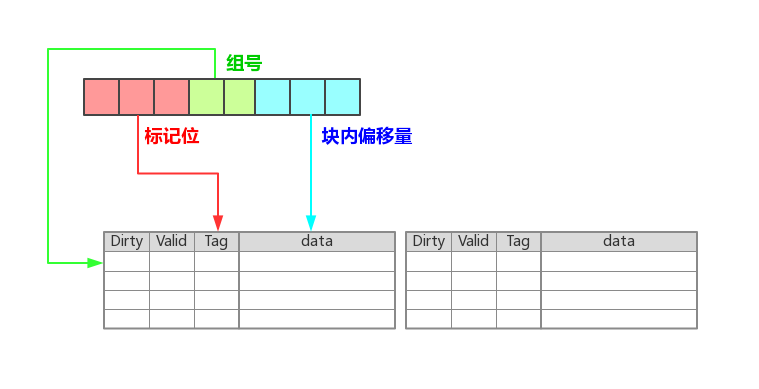
\includegraphics[width =\linewidth]{figure/ex.jpg}
\caption{Cache基本结构示例:块大小$b=64$、组数$S=4$、路数$N=2$}
\end{figure}

\subsection{高速缓存读写}

\noindent
{\bf (1) 如何判断Cache中是否存在我们需要的数据?}

首先,我们先根据访存的地址确定其映射到的组号:
\begin{lstlisting}[language=Verilog]
assign SET_ID = addr[OFFSET + SET_LEN - 1 : OFFSET];
\end{lstlisting} 

之后,我们利用for循环,判断组内是否存在有效行的标记位与访存地址相同,若存在,则说明找到了命中的位置。
\begin{lstlisting}[language=Verilog]
always @(*)
    for (i = 0; i < LINE_CNT; i = i + 1)
      hiti[i] = valid[SET_ID][i] & (tag[SET_ID][i] == addr[8:OFFSET + SET_LEN]);
assign hit = | hiti;
\end{lstlisting} 


\noindent
{\bf (2) 如何控制Cache的读写?}

当Cache命中时,我们可以根据刚刚计算出的hiti数组,对命中的组进行操作:
\begin{itemize}
\item {\bf 读}:
\begin{lstlisting}[language=Verilog]
for (i = 0; i < LINE_CNT; i = i + 1)
  if (hiti[i]) rdata = data[SET_ID][i][addr[OFFSET-1:2]*32 +: 32];
\end{lstlisting}
\item {\bf 写}: 
\begin{lstlisting}[language=Verilog]
for (i = 0; i < LINE_CNT; i = i + 1)
  if (hiti[i])
  begin
    dirty[SET_ID][i] = 1;
    data[SET_ID][i][addr[OFFSET-1:2]*32 +: 32] = wdata;
  end
\end{lstlisting} 
\end{itemize}

\noindent
{\bf (3) 如何与Memory交互?}

当Cache未命中时,我们需要从内存中取数据。这里我们直接套用了原来的Dmem,通过改变写信号与访存地址来获取我们想要的数据。需要注意,我们这里每次访存取出的块大小不再是32,而是给定的参数BLOCK\_SIZE。
\begin{lstlisting}[language=Verilog]    
Dmem #(BLOCK_SIZE) dmem(clk, reset, ADDR, WEN, WDATA, RDATA);
\end{lstlisting} 

当发生miss时,我们通过改变地址,来从内存中获取数据:
\begin{lstlisting}[language=Verilog]    
ADDR = {addr[8:OFFSET], 'OFFSET'b0};
WEN = 0;
WDATA = 0;
\end{lstlisting} 

注意,这里我们的Dmem是组合逻辑,所以不存在延时。而访存的延时,我们会通过状态机来设置,这将在下一小节详细讨论。

\subsection{访存延时实现}

为了模拟访存时的时间延时,在每次访存时我们需要让流水线等待几个周期,且根据hit与miss的情况等待不同的周期数。这一点我们可以通过状态机来实现。
\begin{figure}[h]
\centering
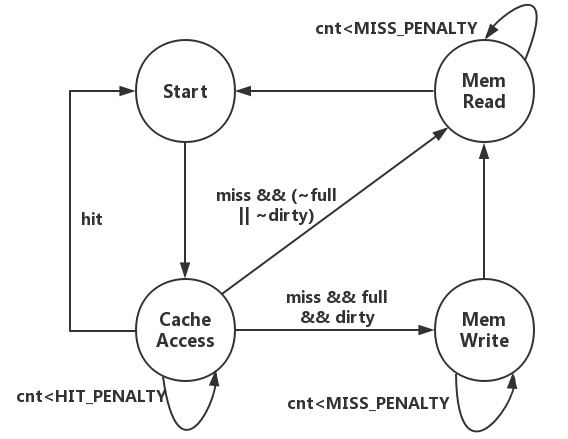
\includegraphics[width = 0.7\linewidth]{figure/state.jpg}
\caption{Cache延时状态机}
\end{figure}

首先,我们需要设置两个延时参数:HIT\_PENALTY和MISS\_PENALTY,分别表示从cache中取数据和从memory中取数据需要的周期数。

之后,设计四个状态,含义如下:
\begin{enumerate}
\item {\bf Start}: 起始状态。若指令不需要访存,则始终停留在该状态;若需要访存时,从该状态起始,对计数器清零。
\item {\bf CacheAccess}: 访问Cache的状态,自带一个计数器。当计数器累加到HIT\_PENALTY时,根据是否hit,选择转移到的状态。\\
{\bf (1)} 若{\em 命中},则从Cache中将数据取出,并转移回Start状态,标记为取数据完成。\\
{\bf (2)} 若{\em 未命中且当前组已满且需要写入},则下一步需要根据替换策略进行替换,跳至MemWrite状态,并将计数器清零。\\
{\bf (3)} 若{\em 未命中且当前组仍有空位},则下一步从内存中取数据,跳至MemRead状态,并将计数器清零。
\item {\bf MemWrite}: 写内存状态,当需要进行替换时,进入该状态。在状态起始,更改访存的地址和写数据,设置写使能为1。当计数器累加到MISS\_PENALTY时,将其清零,跳至MemRead状态。
\item {\bf MemRead}: 读内存状态,从内存中读取需要的数据。在状态起始,将访存的地址设置为输入的地址信号。当计数器累加至MISS\_PENALTY时,将其清零,输出读出的数据,并标记为取数据完成,跳至Start状态。
\end{enumerate}

\subsection{替换策略实现}

\paragraph{随机替换(RAND)}

\paragraph{先进先出(FIFO)}

\paragraph{最不常使用(LFU)}

\paragraph{最近最少使用(LRU)}

\subsection{流水线结构调整}
\label{sec:pipe}

整个流水线的变动并不大,主要调整在暂停信号。当数据未取完时,需要将流水线完全暂停住。我们可以通过增加两个信号来控制:LW信号控制是否为lw或sw指令、DATA\_COMPLETE信号控制是否完成取数据操作。

在冒险处理Hazard模块中,若当前Memory阶段的指令为lw或sw指令,且未完成取数据操作,则令整个流水线暂停,设置所有状态寄存器的Stall信号为1即可。


\newpage
\section{测试样例与结果}

与单周期相同的测试样例均已通过,这里只列举几个关键的和新加入的测试样例。

\subsection{swlw.in}

\begin{lstlisting}
 0x0 : addi $s0, $0, 0      | 20100000
 0x4 : addi $t0, $0, 0      | 20080000
 0x8 : addi $v1, $0, 10     | 2003000a
 0xc : for:                 | 
 0xc : sw $t0, 0($s0)       | ae080000
0x10 : addi $t0, $t0, 1     | 21080001
0x14 : addi $s0, $s0, 4     | 22100004
0x18 : bne $t0, $v1, for    | 1468fffc
0x1c : addi $s0, $0, 0      | 20100000
0x20 : addi $t0, $0, 0      | 20080000
0x24 : addi $t1, $0, 0      | 20090000
0x28 : addi $s1, $0, 0      | 20110000
0x2c : for2:                | 
0x2c : lw $t0, 0($s0)       | 8e080000
0x30 : add $s1, $s1, $t0    | 02288820
0x34 : addi $s0, $s0, 4     | 22100004
0x38 : addi $t1, $t1, 1     | 21290001
0x3c : slt $v0, $v1, $t1    | 0069102a
0x40 : beq $v0, $0, for2    | 1002fffa
0x44 : nop                  | 00000000
0x48 : nop                  | 
\end{lstlisting} 


\newpage
\section{Cache性能实验}


\newpage
\section{注意事项}

\subsection{遇到的问题}

\begin{enumerate}
\item 对Dmem的初始化如果放在initial中好像会有些问题,我把它调整为reset为1时进行初始化就好了。
\item 仿真的结果和在板子上的结果可能会差异很大,在同一个时钟沿,仿真时两个信号会同时变化,而在板子上就不是了。可以通过将信号分别调整为上升沿和下降沿触发来解决该问题。
\end{enumerate}

\section{申A理由}

\begin{itemize}
\item 实现了参数化的高速缓存,复用性强
\item 设计检验Cache正确性与性能的汇编代买
\item 进行了大量实验,对比不同大小与替换策略Cache的性能
\end{itemize}

\section{致谢}

感谢罗翔同学与我进行深入的讨论,对实验的设计提出了宝贵的建议!

\end{sloppypar}
\end{document}
